
\begin{table}[t]
\caption{Comparison of fast sampling methods on CIFAR-10 for diffusion models in the literature. The FID score is computed with the original FID implementation to compare with the other methods. NFE: number of function evaluations.}
\label{tb:fid_cifar}
\vskip 0.1in
\begin{center}
\begin{small}
\begin{tabular}{lccc}
\toprule
Method & NFE & FID & Model size \\
\midrule
Ours    & 1 &  \textbf{3.78} & 65.8M   \\ 
\midrule
Knowledge distillation\\\cite{luhman2021knowledge}  & 1 & 9.36 & 35.7M\\
\midrule
Progressive distillation\\\cite{salimans2021progressive}    & 1 & 9.12 & 60.0M  \\
        & 2 & 4.51  & \\
        & 4 & 3.00  & \\ 
\midrule 
LSGM~\cite{vahdat2021score} & 147 & 2.10  & 475.0M\\
\midrule
GGDM + PRED + TIME\\ \cite{watson2021learning}                      & 5                 & 13.77   &  35.7M  \\
                                         & 10                 & 8.23    &   \\ 
\midrule
DDIM~\cite{song2020denoising}   & 10                & 13.36   &  35.7M \\ 
                                & 20           & 6.84   &   \\
                                & 50 & 4.67 & \\
\midrule 
SN-DDIM~\cite{bao2022estimating} & 10 & 12.19 & 52.6M \\ 
\midrule 
FastDPM~\cite{kong2021fast} & 10    & 9.90 & 35.7M \\ 
\midrule
DPM-solver~\cite{lu2022dpm} & 10 & 4.70 & 35.7M\\ 
\midrule 
DEIS~\cite{zhang2022fast} & 10 & 4.17 & - \\
\toprule 
\textbf{Diffusion + GAN} \\
\midrule
TDPM~\cite{zheng2022truncated} & 5 & 3.34 & 35.7M\\
DDGAN~\cite{xiao2021tackling} & 4 & 3.75 & - \\
% add LSGM, 
\bottomrule
\end{tabular}
\end{small}
\end{center}
\vskip -0.05in
\end{table}
\section{Experiments}
In our experiments, we examine the proposed method on both unconditional and conditional image generation tasks.
% , which are known as one of the most challenging settings for diffusion model sampling in the literature. 
We show that our method dramatically accelerates the sampling process of diffusion models, compared to existing fast sampling methods including both training-free and training-based approaches. Our code is available at \href{https://github.com/devzhk/DSNO-pytorch}{https://github.com/devzhk/DSNO-pytorch}. 

\begin{table*}[t]
\caption{Comparison of fast sampling methods on class-conditional ImageNet-64 for diffusion models in the literature. The results of DDIM and EDM are reported by \citet{karras2022elucidating} using the pre-trained model \cite{dhariwal2021diffusion}.}
\label{tb:fid_imagenet}
\vskip 0.1in
\begin{center}
\begin{small}
\begin{tabular}{lcccc}
\toprule
Method & Model evaluations & FID score & Recall & Model size\\
\midrule
Ours    & 1 &  \textbf{7.83} & \textbf{0.61} & 329.2M\\
\midrule
Progressive distillation~\cite{salimans2021progressive}    & 1 & 15.99 & 0.60 &  295.9M\\
        & 2 & 7.11 & 0.63 & \\
        & 4 & 3.84 &  0.63 & \\ 
% \midrule
% GGDM + PRED + TIME~\cite{watson2021learning} & 25 & 18.40 & - & 295.9M \\
\midrule
EDM~\cite{karras2022elucidating}                   &  79                 & 2.44  & 0.67   &  295.9M\\
\midrule
DDIM~\cite{song2020denoising}   & 32                & 5.00   & -  & 295.9M \\
\midrule
BigGAN-deep~\cite{brock2018large} & 1 & 4.06 & 0.48 & \\
ADM~\cite{dhariwal2021diffusion} & 250 & 2.07 & 0.63 & 295.9M \\ 
% \midrule 
% SN-DDIM~\cite{bao2022estimating} & 100 & 17.53 & 121.5M \\ 
\bottomrule
\end{tabular}
\end{small}
\end{center}
\vskip -0.1in
\end{table*}



\begin{table}[t]
\caption{One model evaluation cost tested on V100. We compare the time cost of a single forward pass of DSNO and the corresponding original backbone. The reported results are averaged over 20 runs. The baseline models are from~\citet{salimans2021progressive}.}
\label{tb:speed_cifar}
\begin{center}
\begin{small}
\begin{tabular}{lccc}
\toprule
Backbone & Runtime & Model size \\
\midrule
CIFAR-10   & 0.033s & 60.00M \\
 DSNO-CIFAR-10 (ours)   & 0.050s & 65.77M\\
 \midrule
ImageNet64   & 0.066s & 295.90M  \\
DSNO-ImageNet-64 (ours) & 0.080s &  329.23M\\
\bottomrule
\end{tabular}
\end{small}
\end{center}
\vskip -0.1in
\end{table}


\subsection{Experimental setup}
We first randomly sample a training set of ODE trajectories using the pre-trained diffusion model to be distilled. 
% and only save 9 steps including the initial condition to disk for each trajectory.  
We then build the network backbone for DSNO by simply adding the proposed temporal convolution layers to the above diffusion model. We initialize the modules from the existing architecture  with the pre-trained weights. 
As for the activation function in the temporal convolution layer, we use the leaky rectified linear unit (LeakyReLU) for $\sigma$.
We mainly use $\ell^1$ loss for the experiments on CIFAR10 and ImageNet-64. We also experiment with LPIPS~\cite{zhang2018unreasonable} loss on CIFAR10 like one concurrent work~\cite{song2023consistency} does. Regarding the choice of the loss weighting function, we set $\lambda(t) = \frac{\alpha_t}{\sigma_t}$, which is the square root of the SNR loss weighting used in the original diffusion model~\cite{salimans2021progressive}. We take the square root because our loss function is not squared. 
We use a batch size of 256 for CIFAR-10 experiments, a batch size of 2048 for ImageNet experiments, and a batch size of 128 by default in our ablation study. We use the same base learning rate of 0.0002, learning rate warmup schedule, and $\beta_1,\beta_2$ of Adam~\cite{kingma2014adam} as used in the diffusion model training without tuning these hyperparameters. 
\vspace{-0.1in}
\paragraph{Evaluation metric}
We use the Frechet inception distance (FID) \cite{heusel2017gans} to evaluate the quality of generated images. FID score is computed by comparing 50,000 generated images against the corresponding reference statistics of the dataset.  We use the ADM’s TensorFlow evaluation suite~\citep{dhariwal2021diffusion} and EDM's evaluation code~\cite{karras2022elucidating} to compute FID-50K with the same reference statistics. We also report Recall~\cite{kynkaanniemi2019improved} as the secondary metric of mode coverage for the experiments on ImageNet-64. 


\subsection{Unconditional generation: CIFAR-10}

\paragraph{Trajectory data collection.} We first generate 1 million trajectories with 512-step DDIM \cite{song2020denoising} using the pre-trained diffusion model proposed by~\citet{salimans2021progressive}, and use it to train DSNO. The FID score of the training set is 2.51, computed over the first 50k data points in the training set. 
% [need to check ngc for exact number].  
% Running the trajectory generation for CIFAR-10 on 8 V100 GPUs takes less than one day. 

\vspace{-0.1in}
\paragraph{Sampling quality and speed.}
Table~\ref{tb:fid_cifar} compares the proposed DSNO trained with a temporal resolution of 4 against both training-based and training-free sampling methods in terms of FID and the corresponding number of model evaluations. DSNO clearly outperforms all the baselines with only one model evaluation and even achieves a better FID score than 2-step progressive distillation models. Furthermore, we compare the cost of one single forward pass of both DSNO and the original backbone\footnote{The progressive distillation only has JAX implementation. We implement its backbone in Pytorch and port the pre-trained weights from the official JAX checkpoint so that we can make a fair speed comparison within the same framework. } on a V100 in a standard AWS p3.2xlarge instance. For the speed test, we do 20 warm-up runs to avoid the potential inconsistency arising from the built-in cudnn autotuner. Since the time cost of progressive distillation grows linearly with the number of sampling steps, we can easily calculate the speedup of DSNO over the progressive distillation from Table~\ref{tb:speed_cifar}. DSNO is 2.6 times faster than the 4-step progressive distillation model and 1.3 times faster than 2-step progressive distillation model. Compared to hybrid models that combine GAN and diffusion models, DSNO achieves comparable performance with at most one-fourth number of model evaluations. 

% \vspace{-0.1in}
% \paragraph{Model size and training cost.} The original architecture of the diffusion model contains 60,004,099 parameters. DSNO contains 65,771,267 parameters, which increases by less than 10\% in model size. The training for CIFAR-10 takes 3-4 days on a single node with 8 V100 GPUs.



% \begin{figure*}[t]
%         \centering
%         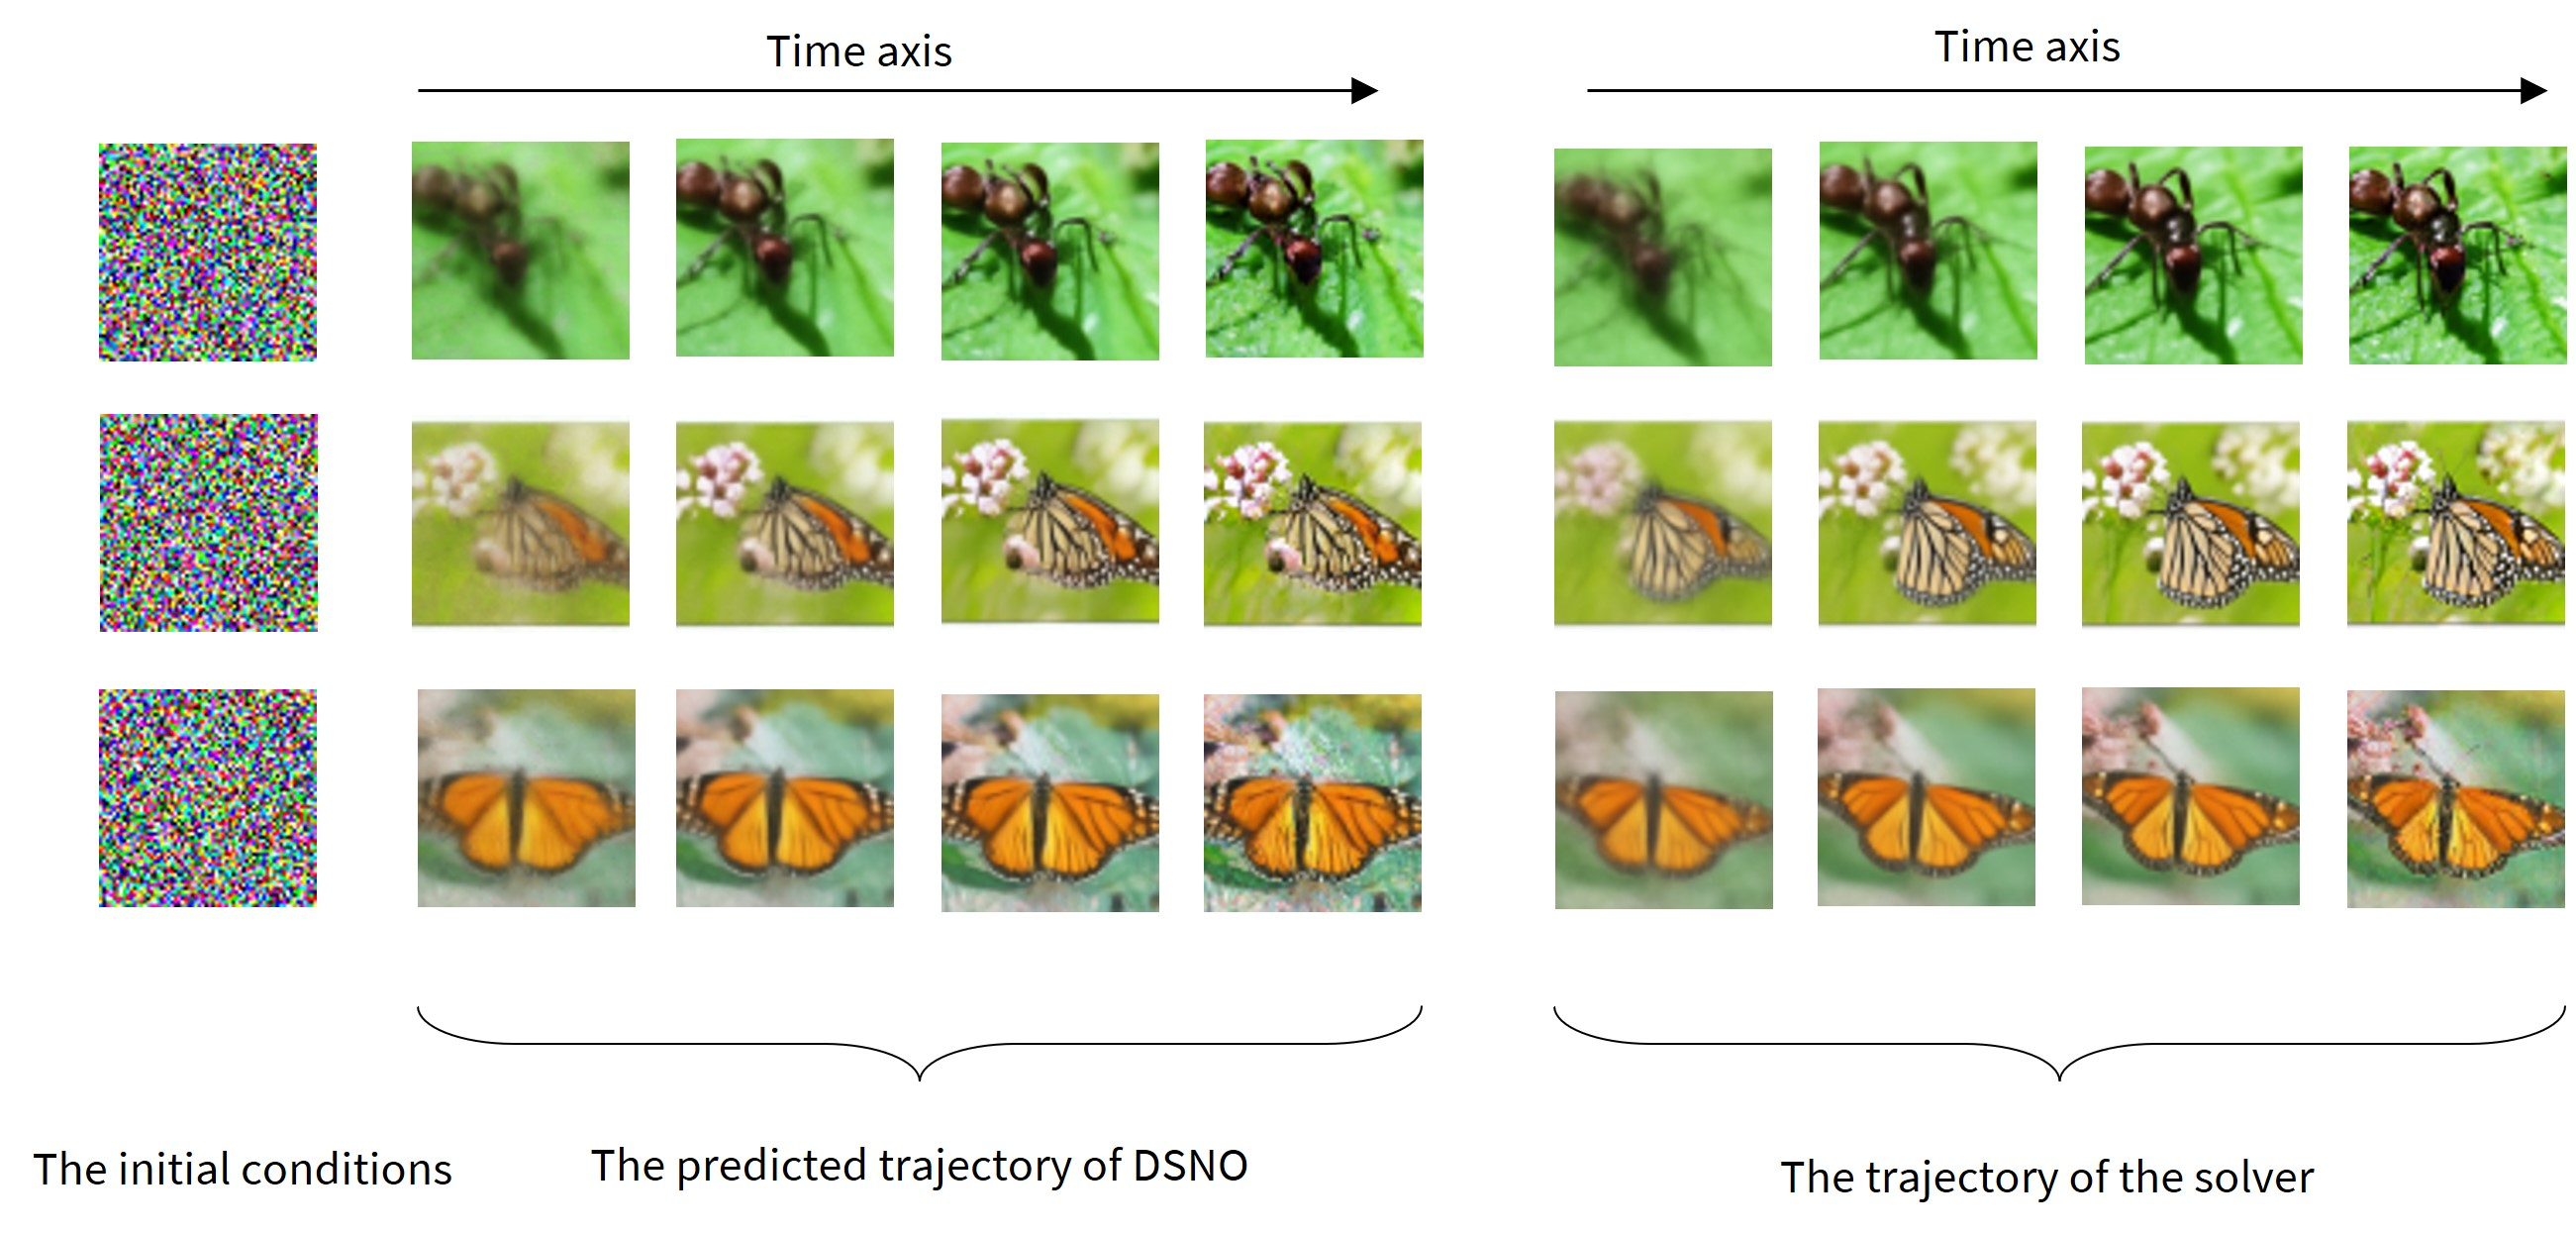
\includegraphics[width=0.97\columnwidth]{figs/demo_traj.jpg}
%         \caption{Comparison between the trajectory predicted by DSNO and the trajectory from the original solver on ImageNet-64, for the fixed random seed with a temporal resolution 4. Left: the prediction by DSNO. Right: the trajectory generated by solver. }
%         \label{fig:demo_imagenet_traj}
% \end{figure*}

\begin{figure}[t]
        \centering
        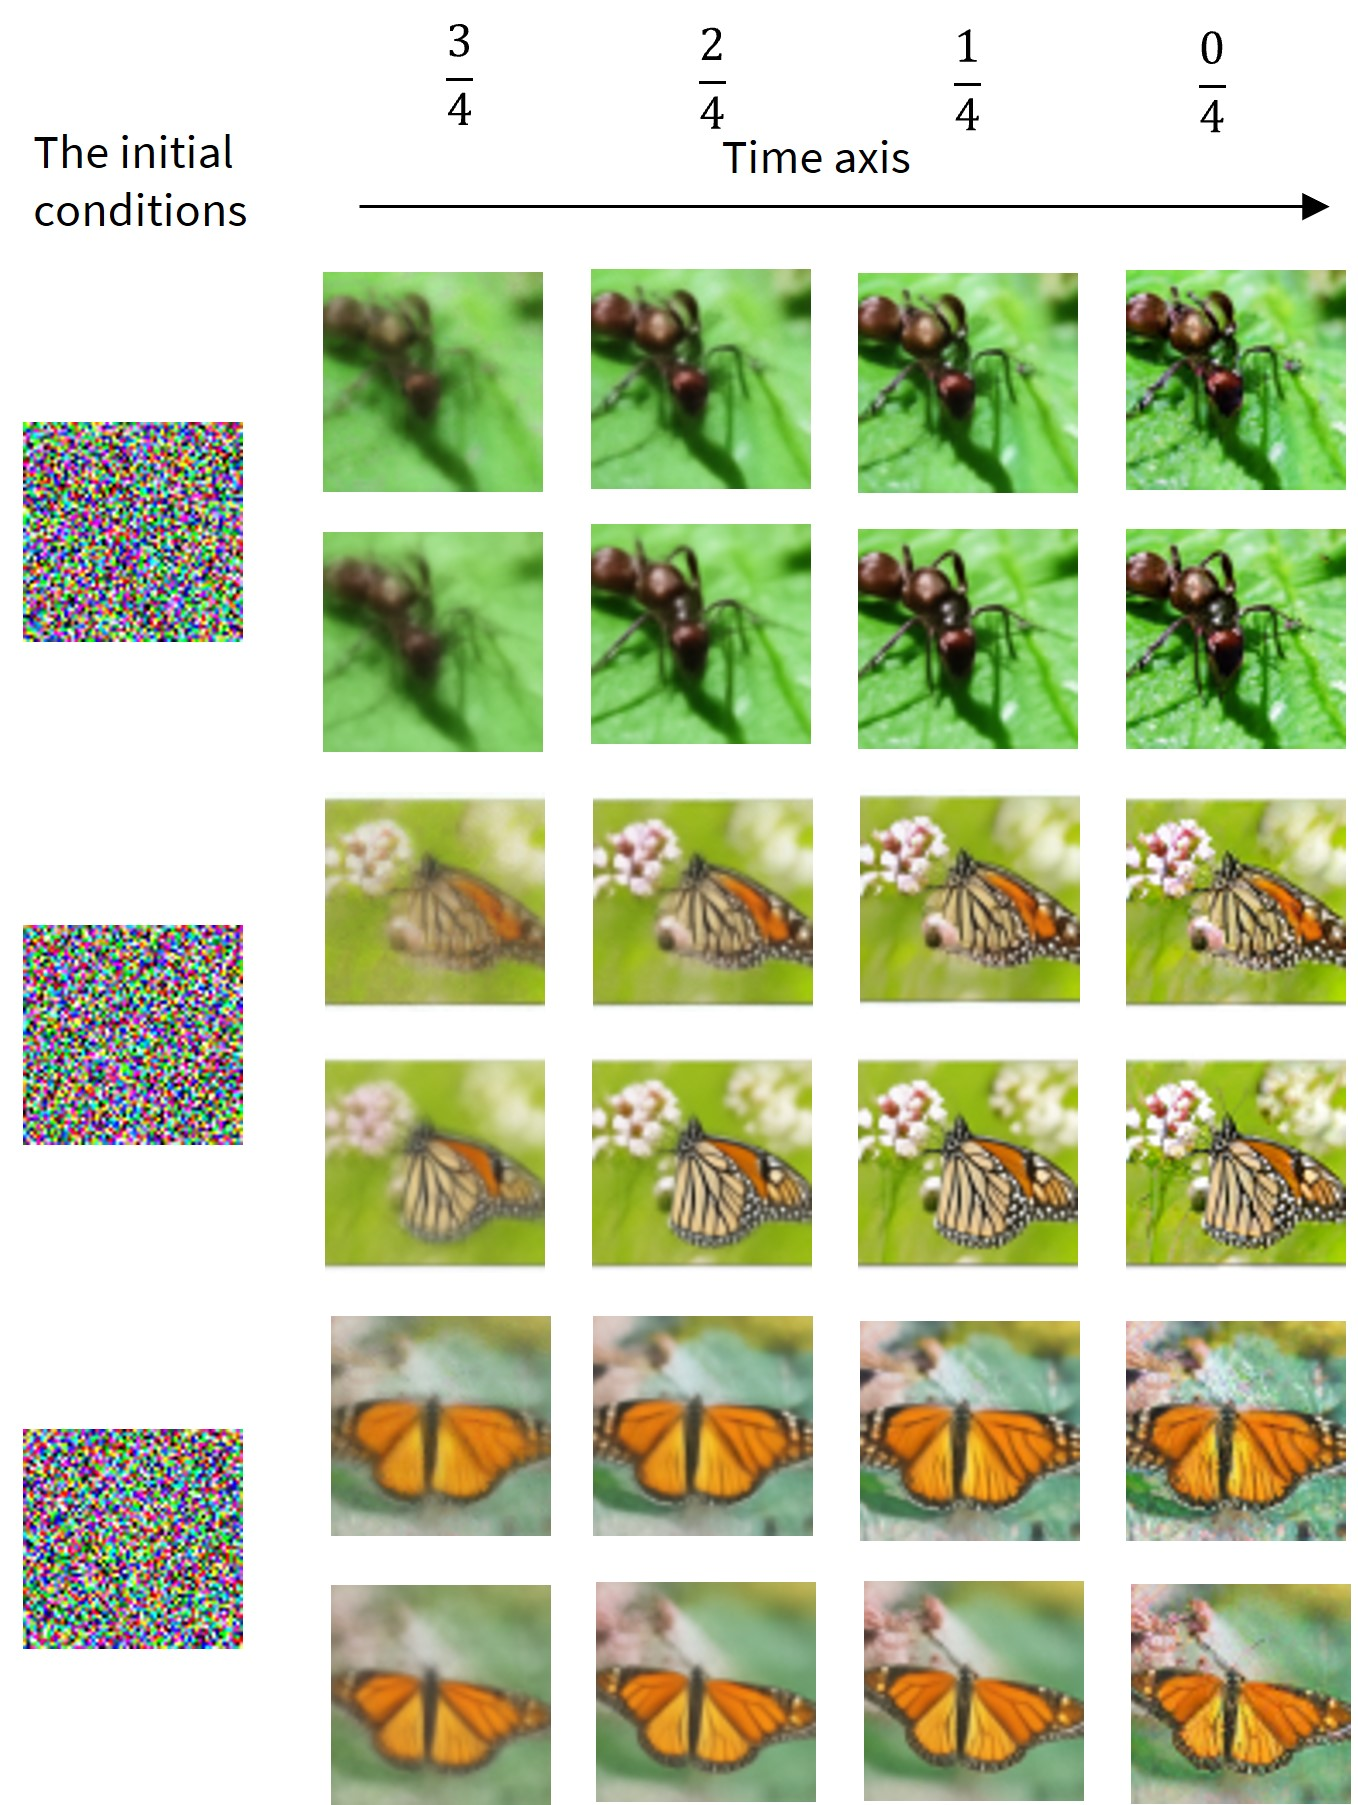
\includegraphics[width=0.97\columnwidth]{figs/demo_traj_1.jpg}
        \vspace{-3pt}
        \caption{Comparison between the trajectory predicted by DSNO and that from the original solver on ImageNet-64, for the fixed random seed with a temporal resolution 4. Upper row: the prediction by DSNO. Lower row: the trajectory generated by solver. }
        \label{fig:demo_imagenet_traj}
        \vspace{-5pt}
\end{figure}

% \begin{figure*}[ht]
%         \centering
%         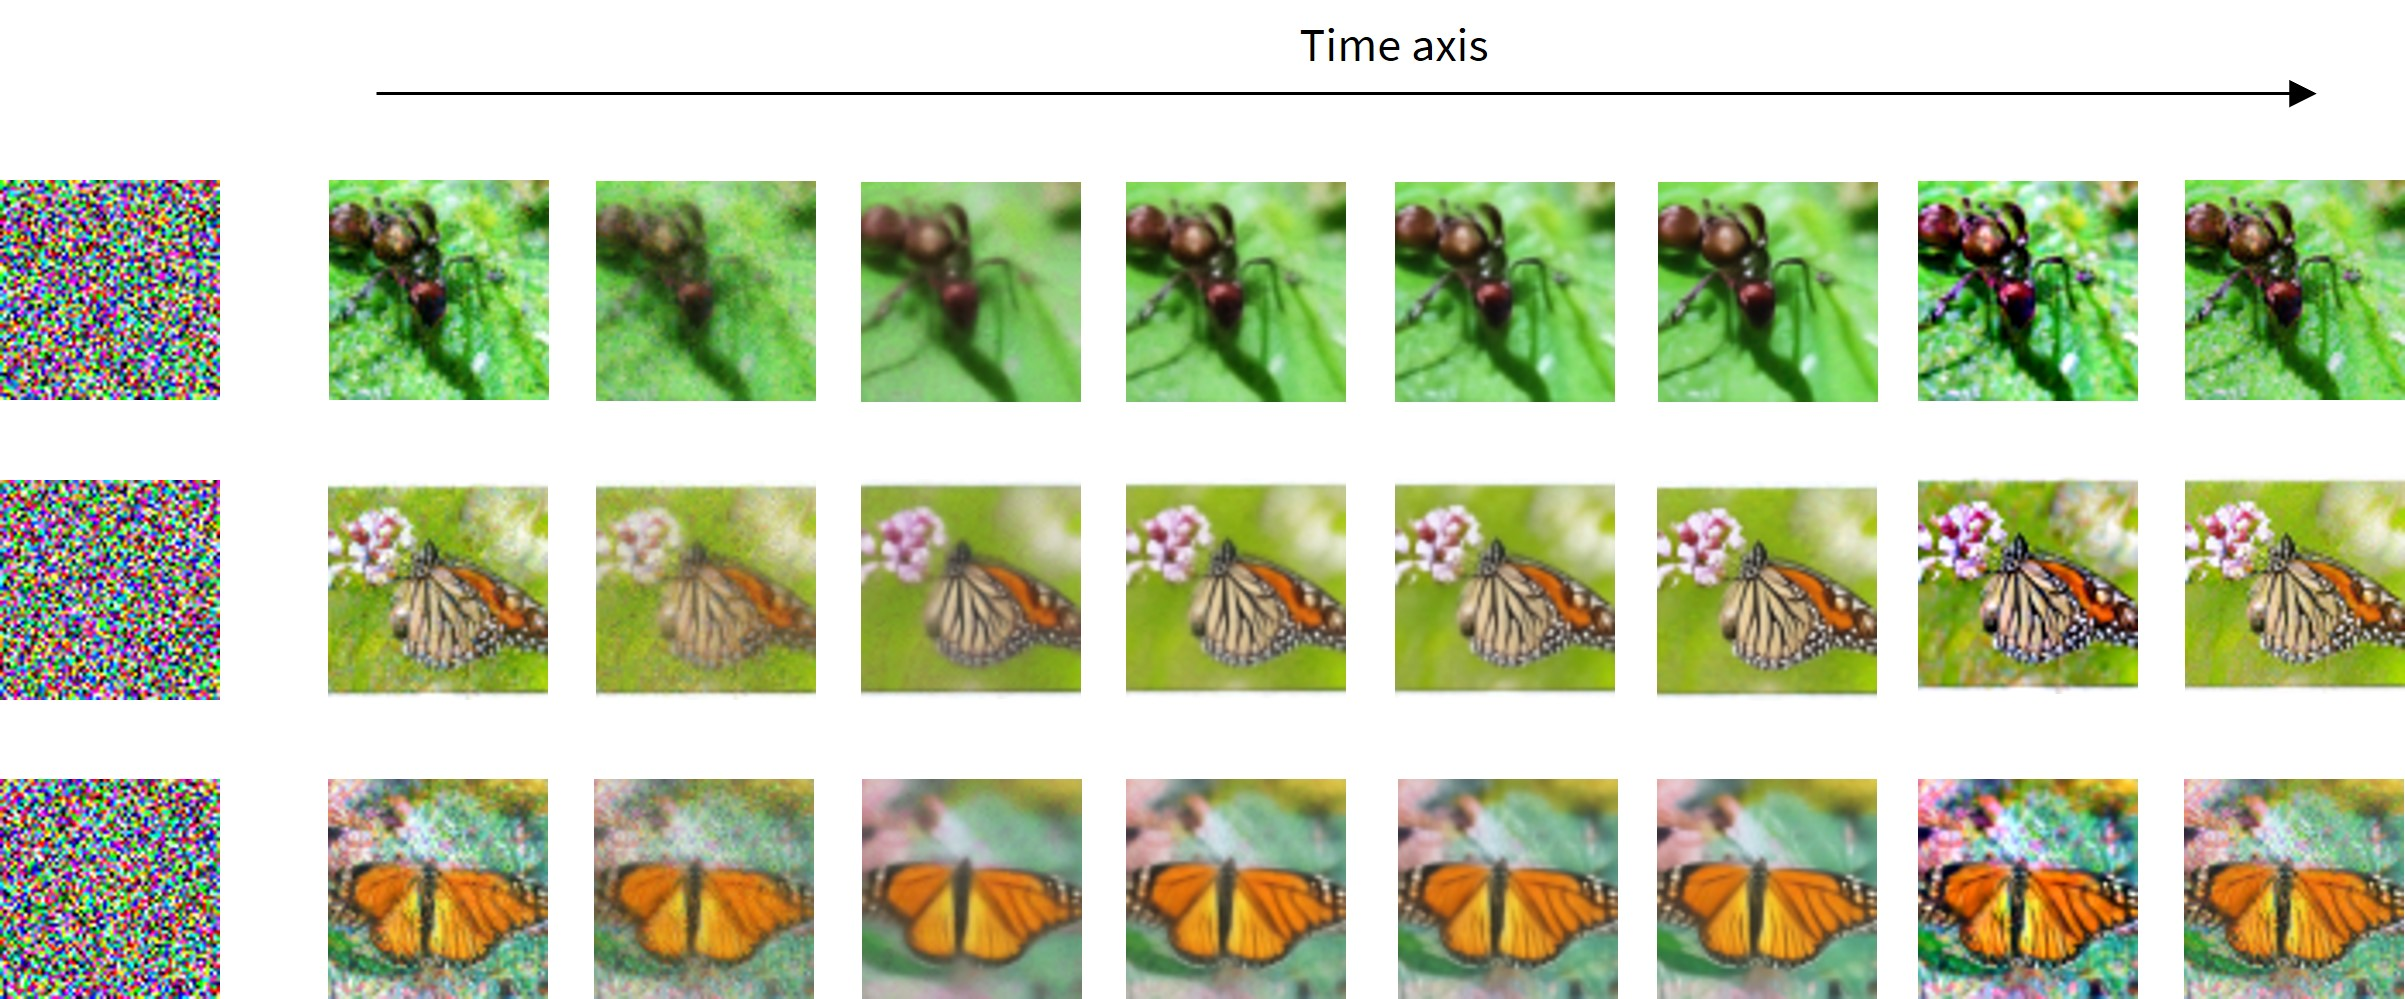
\includegraphics[width=0.75\textwidth]{figs/demo-high-res.jpg}
%         \caption{The predicted trajectory of DSNO in temporal resolution 8 on ImageNet-64. We train the DSNO with temporal resolution 4 and then use it to predict the trajectory with temporal resolution 8. }
%         \label{fig:demo_imagenet}
% \end{figure*}
\subsection{Conditional generation: ImageNet-64}
\paragraph{Trajectory data collection.} We generate 2.3 million trajectories with 16-step progressive distillation \cite{salimans2021progressive} using the pre-trained diffusion model from its official code base. The FID score of the generated training set is 2.70, computed over the first 50k training data points. 
\vspace{-0.1in}
\paragraph{Sampling quality and speed.} Table~\ref{tb:fid_imagenet} compares DSNO trained with a temporal resolution of 4 against the recent advanced fast sampling methods for diffusion models. 
DSNO clearly outperforms 1-step progressive distillation model and archives comparable FID  2-step models of progressive distillation with only one model evaluation. From Table~\ref{tb:speed_cifar}, DSNO has 1.7 times speedup over progressive distillation. The recall of DSNO is comparable to ADM's, showing that DSNO inherits the original diffusion model's diversity/mode coverage as it learns to solve the probability flow ODE. 

% \vspace{-0.1in}
% \paragraph{Model size and training cost.} The original architecture of the diffusion model contains 295,900,035 parameters. DSNO contains 329,225,091 parameters, which increases by around 10\% in model size. Training on ImageNet-64 takes about 7 days on 64 V100 GPUs with mixed precision. 

\vspace{-0.1in}
\paragraph{Trajectory prediction and reconstruction.}
Figure~\ref{fig:demo_imagenet_traj} compares the trajectories predicted by DSNO and the original ODE solver, respectively, for the fixed random seed with a temporal resolution 4. We see that the DSNO predicted trajectory highly matches the groundth-truth ODE trajectory, which demonstrates the effectiveness of DSNO with parallel decoding. Besides, Figure~\ref{fig:demo_imagenet_recon} shows the random samples from DSNO and the original pre-trained diffusion model with the same random seed. It is clear that the mapping from Gaussian noise to the output image is well-preserved.


\begin{figure}[ht]
        \centering
        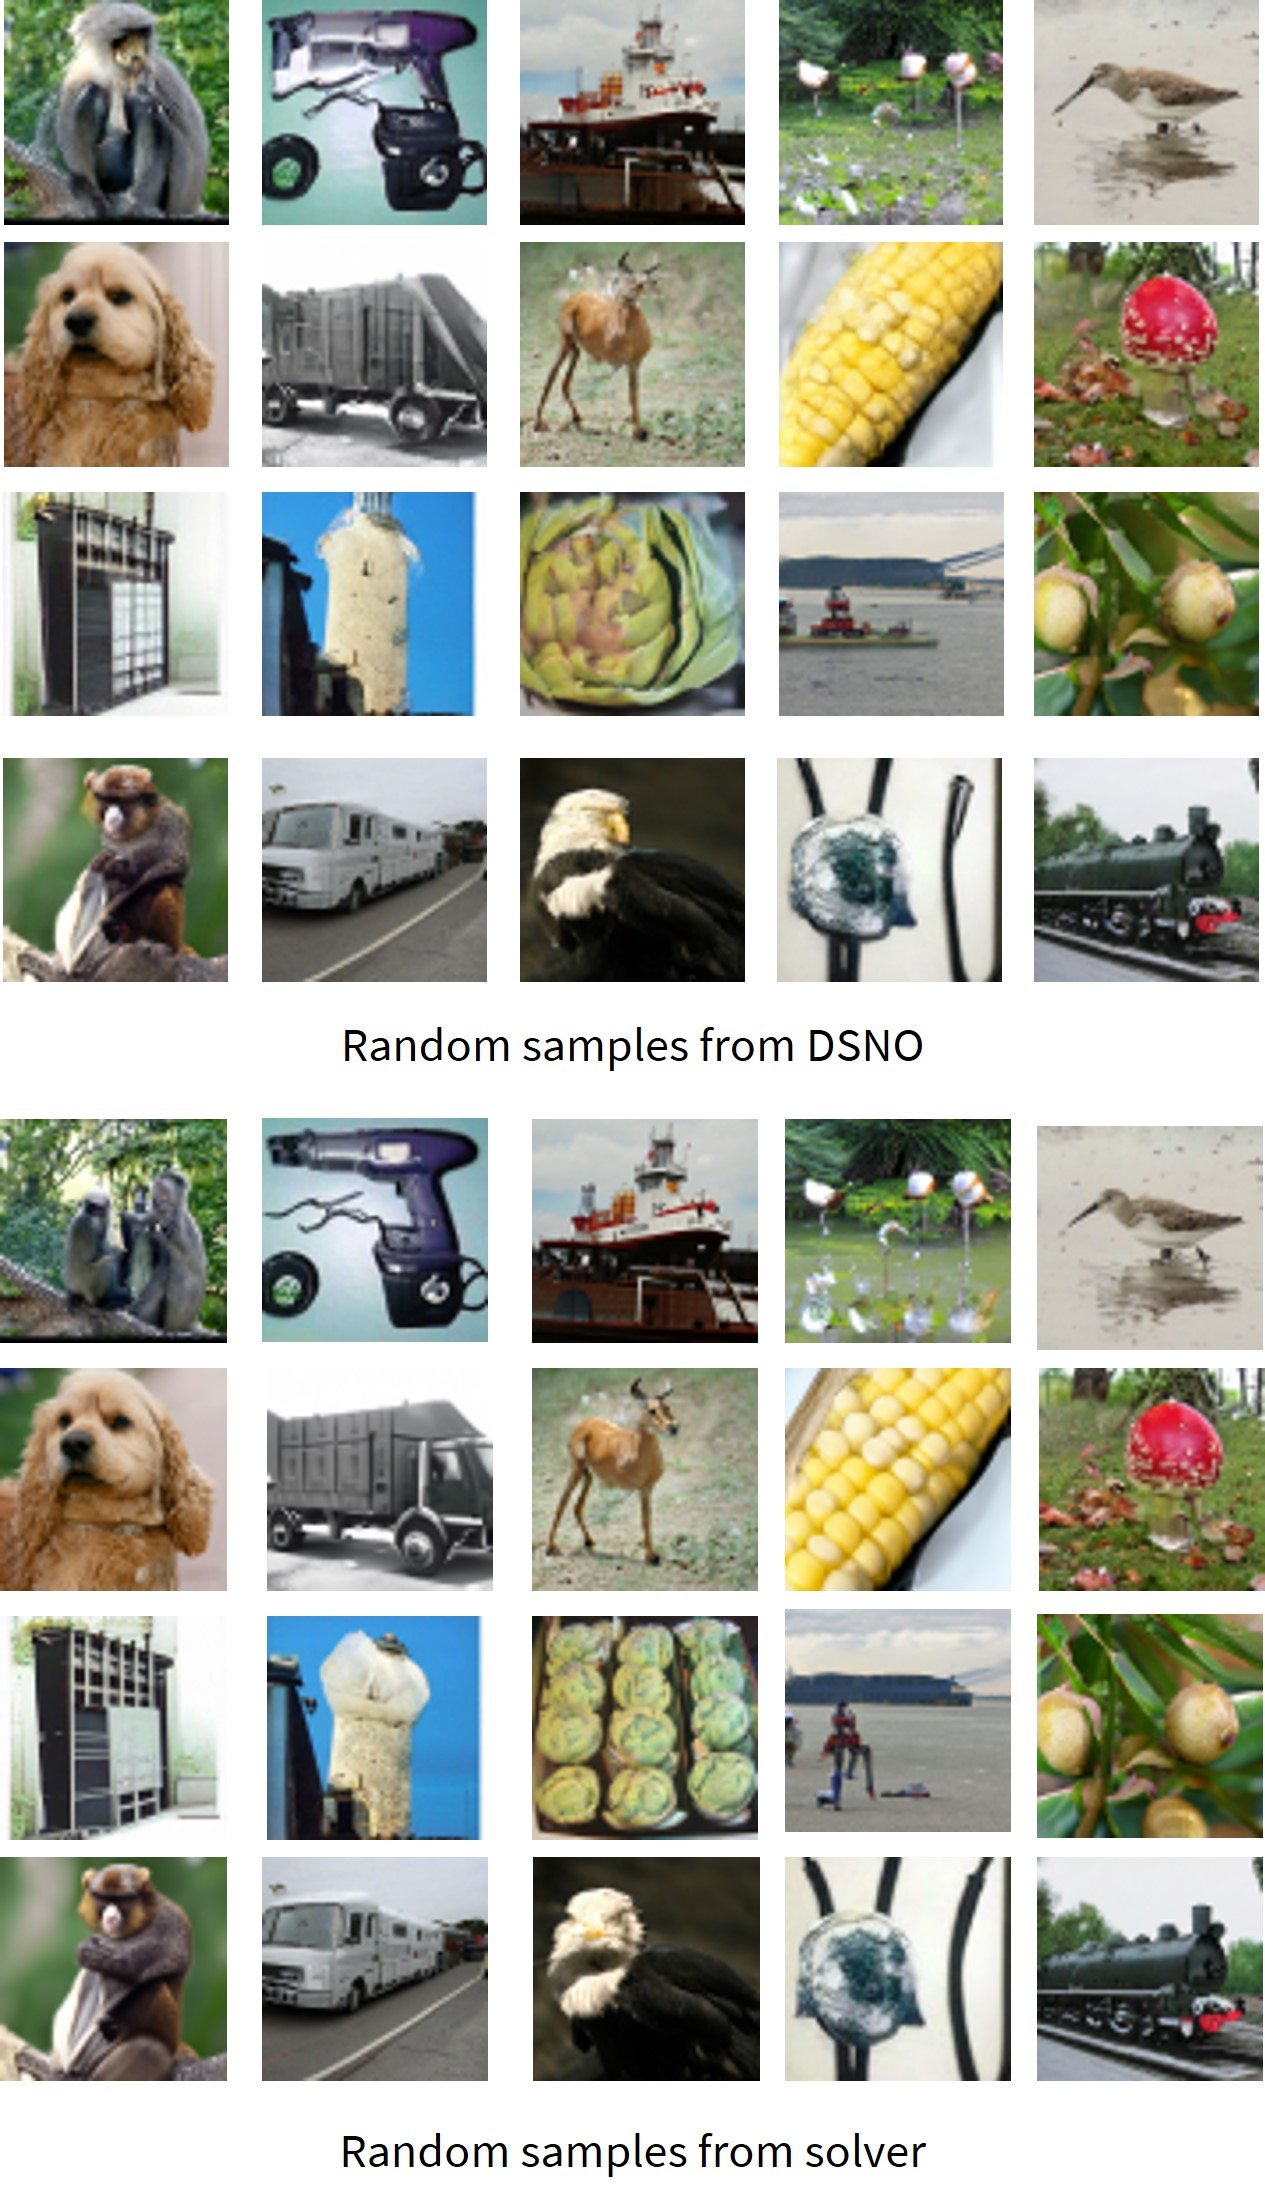
\includegraphics[width=0.8\columnwidth]{figs/demo_images.jpg}
        \caption{Upper panel: random samples generated by DSNO. Bottom panel: generated by the solver. }
        \label{fig:demo_imagenet_recon}
\end{figure}



\begin{table}[ht]
\caption{Impact of temporal convolution. We compare the performance of architectures with and without temporal convolution blocks while keeping all other settings the same. }
\label{tb:cifar_ablation_temporal_conv}
\begin{center}
\begin{small}
\begin{tabular}{lccc}
\toprule
 Training steps & U-Net &  U-Net + Temporal Conv \\
\midrule
300k  & 8.09 & 4.23 \\
400k & 7.85 & 4.12 \\ 
\bottomrule
\end{tabular}
\end{small}
\end{center}
\vskip -0.1in
\end{table}

\begin{table}[ht]
\caption{Ablation study on the choice of training loss weighting and time discretization scheme. The temporal resolution is fixed to 4 in this group of experiments. }
\label{tb:cifar_ablation_loss-weight}
\begin{center}
\begin{small}
\begin{tabular}{lcc}
\toprule
 Loss weighting & Uniform & $\mathrm{SNR}^{0.5}$ \\
% \midrule
FID  & 4.56 & 4.21 \\
\midrule
time discretization scheme & Uniform & Quadratic \\
% \midrule
FID & 4.33 & 4.21 \\
\bottomrule
\end{tabular}
\end{small}
\end{center}
\vskip -0.1in
\end{table}

\begin{table}[ht]
\caption{Ablation study on the choice of the temporal resolution.}
\label{tb:cifar_ablation_resolution}
\begin{center}
\begin{small}
\begin{tabular}{lccc}
\toprule
Temporal resolution & 2 & 4 & 8 \\
\midrule
FID  & 5.01 & 4.21  & 3.98\\
\bottomrule
\end{tabular}
\end{small}
\end{center}
\vskip -0.1in
\end{table}

\subsection{Ablation study}
In this section, we study the effect of different model choices, including the temporal convolution blocks, loss weighting function, temporal resolution, time discretization scheme, and loss function, by performing ablation studies on CIFAR-10. Without stated explicitly, we use batch size 128 and $\ell^1$ norm for the loss function. 
\vspace{-0.1in}
\paragraph{Temporal convolution block.} We first investigate the impact of temporal convolution by comparing the performance of architectures with and without temporal convolution blocks. All the other settings are kept the same such as temporal resolution 4, quadratic time discretization scheme, the square root of the SNR weighting function, and batch size 256. As reported in Table~\ref{tb:cifar_ablation_temporal_conv}, the temporal convolution design is crucial to DSNO's performance as its kernel integration operator nature is a better model inductive bias to model the trajectory in time. 



\vspace{-0.1in}
\paragraph{Loss weighting.}  The loss weighting function used in the training objective of Diffusion models\cite{ho2020denoising, song2020score} typically distributes more weights to the small times, which is important to training diffusion models. We also adopt such a weighting function since it is generally harder to control the error at small times. We observe that such loss weighting function benefits the training of DSNO. As reported in Table~\ref{tb:cifar_ablation_loss-weight}, using the square root of the SNR weighting function slightly improves the FID by 0.35. 
\vspace{-0.1in}
\paragraph{Time discretization scheme.} How to discretize the temporal domain is important to the performance of the numerical solvers. Some small changes to the time discretization scheme could lead to very different sample qualities as shown in~\cite{karras2022elucidating,zhang2022fast}. DSNO also needs to choose a way to discretize the temporal domain. Here we consider the two most common choices of time discretization schemes in the literature: uniform time step and quadratic time step. As shown in Table~\ref{tb:cifar_ablation_loss-weight}, the quadratic time step is slightly better than the uniform time step by 0.12, showing that DSNO is not sensitive to the different time discretization schemes used in the existing solvers and can work nicely with different solvers. 
\vspace{-0.1in}
\paragraph{Temporal resolution.} We study the effect of temporal resolution (i.e., the discretization steps $M$), given the square root of SNR weighting function and the quadratic time discretization scheme. 
% We train different models with temporal resolutions ranging from 2 to 8 with the model parameter $J$ set to half of the resolution. 
As reported in Table~\ref{tb:cifar_ablation_resolution}, the FID improves as we increase the temporal resolution. Since the higher temporal resolution introduces more supervision into the training, it is reasonable to expect better FID scores. However, higher resolution also results in higher computation costs. Since increasing the resolution from 4 to 8 only provides a marginal benefit (due to the compact spectrum we observed in Appendix~\ref{sec:spectrum}), one may use temporal resolution 4 for better efficiency.   

\begin{table}[ht]
\caption{Ablation study on the choice of the loss function. For LPIPS, we use the original VGG-based version without any calibration~\cite{zhang2018unreasonable}.}
\label{tb:cifar_ablation_loss}
\begin{center}
\begin{small}
\begin{tabular}{lcc}
\toprule
Loss function & $\ell^1$ & LPIPS \\
\midrule
FID   & 4.12  & 3.78 \\
\bottomrule
\end{tabular}
\end{small}
\end{center}
\vskip -0.1in
\end{table}
\paragraph{Loss function.} We only vary the loss function but keep the other settings the same, including a batch size of 256, a temporal resolution of 4, and a quadratic discretization scheme.  As shown in Table~\ref{tb:cifar_ablation_loss}, using the original VGG-based LPIPS loss~\cite{zhang2018unreasonable} instead of the standard $\ell^1$ loss leads to a further improvement in the FID score. 
% Table~\ref{tb:cifar_ablation_loss-weight} reports the results of our ablation study. We observe that higher resolution provides stronger supervision and improves the sample quality. Further increasing resolution from 4 to 8 obtains marginal benefit. The quadratic time discretization scheme and $1/\sigma_t$ loss weighting are two common heuristics used in diffusion models. Our experiments show using the same time discretization scheme and loss weighting as used in diffusion model training improves the sample quality. 

% \begin{figure}[ht]
%         \centering
%         \includegraphics[width=0.8\columnwidth]{figs/cifar_ablation_tr.pdf}
%         \caption{FID score of generated samples versus the temporal resolution of the model. }
%         \label{fig:cifar_ablation}
% \end{figure}




